\documentclass[12pt]{article}
\usepackage[margin=1in]{geometry}
\setlength{\headheight}{14.49998pt}
\usepackage{graphicx}
\usepackage{float}
\usepackage{amsmath}
\usepackage{amsfonts}
\usepackage{amssymb}
\usepackage{xcolor}
\usepackage{listings}
\usepackage{tikz}
\usetikzlibrary{automata, positioning}
\usepackage{url}
\usepackage{hyperref}
\usepackage{fancyhdr}
\usepackage{titlesec}
\titlelabel{}
\renewcommand{\thesection}{}
\renewcommand{\thesubsection}{}
\renewcommand{\thesubsubsection}{}
\setcounter{secnumdepth}{0}

% Set up code listings
\lstset{
    basicstyle=\ttfamily\footnotesize,
    breaklines=true,
    frame=single,
    numbers=left,
    numberstyle=\tiny,
    showstringspaces=false,
    commentstyle=\color{gray},
    keywordstyle=\color{blue},
    stringstyle=\color{red}
}

% Header and footer
\pagestyle{fancy}
\fancyhf{}
\rhead{Cameron Brooks}
\lhead{CS321 Assignment 1}
\cfoot{\thepage}

% Title formatting
\titleformat{\section}{\Large\bfseries}{\thesection}{1em}{}
\titleformat{\subsection}{\large\bfseries}{\thesubsection}{1em}{}
\titleformat{\subsubsection}{\normalsize\bfseries}{\thesubsubsection}{1em}{}

\title{Assignment 1: Mathematical Preliminaries and DFAs}
\author{Cameron Brooks \\
        CS321 Introduction to Theory of Computation \\
        Assignment 1}
\date{Wednesday, October 2, 2025}

\begin{document}

\maketitle
\thispagestyle{empty}

\newpage
\tableofcontents
% NOTE: TOC will be empty in this template because sections use placeholder names.
% When pdf-builder agent replaces section titles with actual content (e.g., "Section 1.1: Mathematical Preliminaries"),
% the TOC will automatically populate. Sections are unnumbered but still appear in TOC with their full text.
\newpage

% ============================================
% CONTENT SECTIONS - FILLED BY PDF-BUILDER
% ============================================
% NOTE: The pdf-builder agent should replace:
%   - Section titles (e.g., "Section X.X" → "Section 1.1: Mathematical Preliminaries")
%   - Question numbers and types
%   - [Placeholder text] with actual answers
%   - Image paths (images/placeholder_qX.png → actual screenshot paths)
%   - Figure captions with actual test cases
% ============================================

\section{Section X.X}

\subsection{Question 1 - Example: Proof by Induction}
\textbf{Question:} [Question text will be inserted here by pdf-builder agent]

\textbf{Answer:}

This is an example of how to format a proof by induction. The pdf-builder agent will replace this with actual content.

\textbf{Base case:} State the base case clearly and prove it holds.

\textbf{Inductive hypothesis:} Assume the property holds for some value $k$.

\textbf{Inductive step:} Show that if the property holds for $k$, it must hold for $k+1$.

Therefore, by mathematical induction, the property holds for all values.

% ============================================

\section{Section Y.Y}

\subsection{Question 2 - Example: DFA Construction}
\textbf{Question:} [Question text will be inserted here by pdf-builder agent]

\textbf{Answer:}

This is an example of how to describe a DFA construction. The pdf-builder agent will replace this with actual content.

\textbf{State Description:}
\begin{itemize}
\item $q_0$: [Description of what this state represents]
\item $q_1$: [Description of what this state represents]
\item Additional states as needed...
\end{itemize}

\textbf{Transition function:}
\begin{itemize}
\item From $q_0$: transitions listed here
\item From $q_1$: transitions listed here
\item Additional transitions as needed...
\end{itemize}

[Explanation of why this DFA is correct]

\begin{figure}[H]
\centering
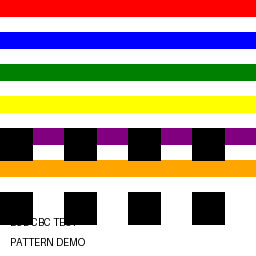
\includegraphics[width=0.85\textwidth]{images/placeholder_q2.png}
\caption{[Caption describing the DFA/automaton and test cases - Accept: [list] | Reject: [list]]}
\label{fig:question_X}
\end{figure}

% ============================================

\subsection{Question 3 - Example: Proving Language Regularity}
\textbf{Question:} [Question text will be inserted here by pdf-builder agent]

\textbf{Answer:}

This is an example of how to prove a language is regular. The pdf-builder agent will replace this with actual content.

To show that the language is regular, we can use one of these approaches:
\begin{itemize}
\item \textbf{DFA Construction:} Construct a DFA that accepts exactly the strings in the language
\item \textbf{Regular Expression:} Provide a regular expression that generates the language
\item \textbf{Closure Properties:} Show the language can be built from simpler regular languages using closure operations
\end{itemize}

[Detailed proof goes here]

\begin{figure}[H]
\centering

\includegraphics[width=0.85\textwidth]{images/placeholder_q3.png}
\caption{[Caption describing the automaton/proof with test cases - Accept: [list] | Reject: [list]]}
\label{fig:question_Y}
\end{figure}

% ============================================

\section{Example: Code Listing Usage}

\subsection{Example 1: JFLAP File Contents}
If you need to show JFLAP XML structure:

\begin{lstlisting}
<?xml version="1.0" encoding="UTF-8"?>
<structure>
  <type>fa</type>
  <automaton>
    <state id="0" name="q0">
      <x>100.0</x>
      <y>100.0</y>
      <initial/>
    </state>
    <state id="1" name="q1">
      <x>250.0</x>
      <y>100.0</y>
      <final/>
    </state>
    <transition>
      <from>0</from>
      <to>1</to>
      <read>a</read>
    </transition>
  </automaton>
</structure>
\end{lstlisting}

\subsection{Example 2: Test Cases}
\textbf{Test Cases Run:}

\begin{lstlisting}
Input: b
Result: Accept

Input: aaab
Result: Accept

Input: bbb
Result: Accept

Input: aa
Result: Reject

Input: (empty string)
Result: Reject

Input: ab
Result: Reject
\end{lstlisting}

\subsection{Example 3: Command Line Usage}
\textbf{Opening JFLAP file:}

\begin{lstlisting}[language=bash]
$ java -jar JFLAP.jar Q2_even_a_odd_b.jff
\end{lstlisting}

\end{document}